\documentclass[11pt,pdftex]{scrartcl}
\usepackage[margin=2.5cm]{geometry} 
\usepackage[utf8]{inputenc}
\RequirePackage[T1]{fontenc}
\usepackage[ngerman]{babel}
\usepackage{graphicx}
\usepackage{tabularx}
\usepackage[hidelinks]{hyperref}
\geometry{a4paper}
\parindent 0.0mm
\newcommand{\bs}{\symbol{'134}}
\newcommand{\Cmd}[1]{\texttt{\def\{{\char`\{}\def\}{\char`\}}\bs#1}}
\makeatletter
\newcommand{\verbatimfont}[1]{\renewcommand{\verbatim@font}{\ttfamily#1}}
\makeatother

\title{Dokumentation Rechnungsvorlage}
\author{Christian Graul}
\date{Version 1.1 --- 22. Mai 2015}

\begin{document}
\maketitle{}
\tableofcontents
\verbatimfont{\small}

\vspace{.5cm}

\section{Einleitung}

In dieser Dokumentation werden die wichtigsten Einstellungen und Kommandos der \LaTeX-Rech\-nungs\-vorlage erläutert. Zur Vorlage gehören folgende Dateien:
\begin{description}
\item[rechnung.tex] Quelldatei für das Rechnungsdokument. Diese Datei wird bearbeitet um ein Rechnungsdokument zu erstellen. Sie kann verändert, umbenannt, vervielfältigt und verschoben werden. Letzteres macht eine Anpassung der Pfade zur Styledatei und den Grafiken notwendig.
\item[rechnung.sty] Styledatei mit allgemeinen Einstellungen, Layoutdefinitionen und Kommandos. In dieser Datei können tiefergehende Änderungen der Rechnungsvorlage vorgenommen werden. Sie sollte möglichst nicht verändert werden, um die Funktionalität nicht zu beeinträchtigen.
\item[bk.pdf + wz.pdf] Grafiken für Briefkopf und Wasserzeichen. Beide Dateien können verändert, ersetzt, umbenannt und verschoben werden. Veränderung bzw.~Ersetzung macht eventuell Anpassungen in der Styledatei notwendig (Größe und Lage der Grafik). Bei Umbenennung und Verschiebung müssen die Pfade zu den Grafiken in der Quelldatei angepasst werden.
\item[rechnung.cwl] TeXstudio Konfigurationsdatei für die Autovervollständigung von Kommandos. TeXstudio ist ein freier \LaTeX-Editor und für verschiedene Plattformen verfügbar. Diese Datei muss in das TeXstudio-Konfigurationsverzeichnis kopiert werden:
\begin{itemize}
\item Windows: \%APPDATA\%\textbackslash texstudio 

\vspace{-0.3em}

\item Linux/Unix/Mac: $\sim$/.config/texstudio
\end{itemize} 
\end{description}

Alle nachfolgenden Erläuterungen beziehen sich auf den Umgang mit der Quelldatei.

\section{Dokumentkopf}

\subsection{Dokumentbasis}
Zu Beginn der Vorlage werden grundlegende Einstellungen zum Dokument vorgenommen.

\begin{verbatim}
\documentclass[12pt,pdftex]{scrartcl}
\usepackage[utf8]{inputenc}
\usepackage{style/rechnung}
\end{verbatim}
Mittels \Cmd{documentclass} wird die Dokumentklasse festgelegt. Als wichtige Optionen wird dabei auch die Basisschriftgröße, hier \emph{12pt}, gewählt. Durch entsprechende Anpassung kann diese Schriftgröße verändert werden.

\Cmd{usepackage} lädt Pakete und Styles in das Dokument. Mit dem Paket \emph{inputenc} wird die Kodierung der Datei angegeben. Die \LaTeX-Dateien müssen entsprechend kodiert sein, wobei \emph{utf8} aus Gründen der Plattformunabhängigkeit und des Zeichensatzes am zweckmäßigsten ist.

In der dritten Zeile wird das hier dokumentierte Paket für die Rechnungsvorlage geladen. Dazu muss der relative oder absolute Pfad zur Styledatei angegeben werden. Liegt die Datei im Verzeichnis der Quelldatei, wird beim Aufruf nur der Dateiname \Cmd{usepackage\{rechnung\}} angegeben. Ansonsten wird der Pfad dem Namen vorangestellt. Achtung: Trennzeichen für den Pfad ist das unter Unix übliche /, nicht \textbackslash, wie unter Windows.

\subsection{Einstellungen}

Die folgenden Einstellungen betreffen das Layout der Rechnung.

\begin{verbatim}
% Einstellungen
\briefpapier{ein}{style/bk.pdf}{style/wz.pdf} % ein/aus, Briefkopf, Wasserzeichen
\faltmarken{ein} % ein/aus
\schrifttyp{sans} % sans/roman
\sprache{de} % de/en
\kundentabelle{ein} % ein/aus
\umsatzsteuer{19} % Prozent
\end{verbatim}

Das Kommando \Cmd{briefpapier} hat die drei Argumente \{Schalter\}\{Briefkopfgrafik\}\{Wasser\-zei\-chen\-grafik\}. Die letzten beiden sind Dateipfade und werden, wie der Pfad zur Styledatei oben, im Grunde nur einmal eingetragen. Sie bleiben dann solange unverändert, wie sich die Grafiken oder deren Pfad nicht ändern. Das erste Argument schaltet das Briefpapier, also die Grafiken, \emph{ein} oder \emph{aus}.

Auf gleichem Wege können die Falt- und Lochermarken über das Kommando \Cmd{faltmarken} \emph{ein}- oder \emph{aus}-geschaltet werden.

Beim Schrifttyp kann über \Cmd{schrifttyp} zwischen serifenloser Schrift \emph{sans} oder Serifenschrift \emph{roman} gewählt werden.

Vordefinierte Textteile der Rechnung sind in zwei Sprachen verfügbar. Mit dem Kommando \Cmd{sprache} kann die Sprache bei Bedarf von Deutsch \emph{de} auf Englisch \emph{en} umgestellt werden.

Das Kommando \Cmd{kundentabelle} schaltet die Tabelle mit Kundendaten (Abbildung~\ref{kundentab}) \emph{ein} bzw. \emph{aus}.

\begin{figure}[htbp]
\begin{center}
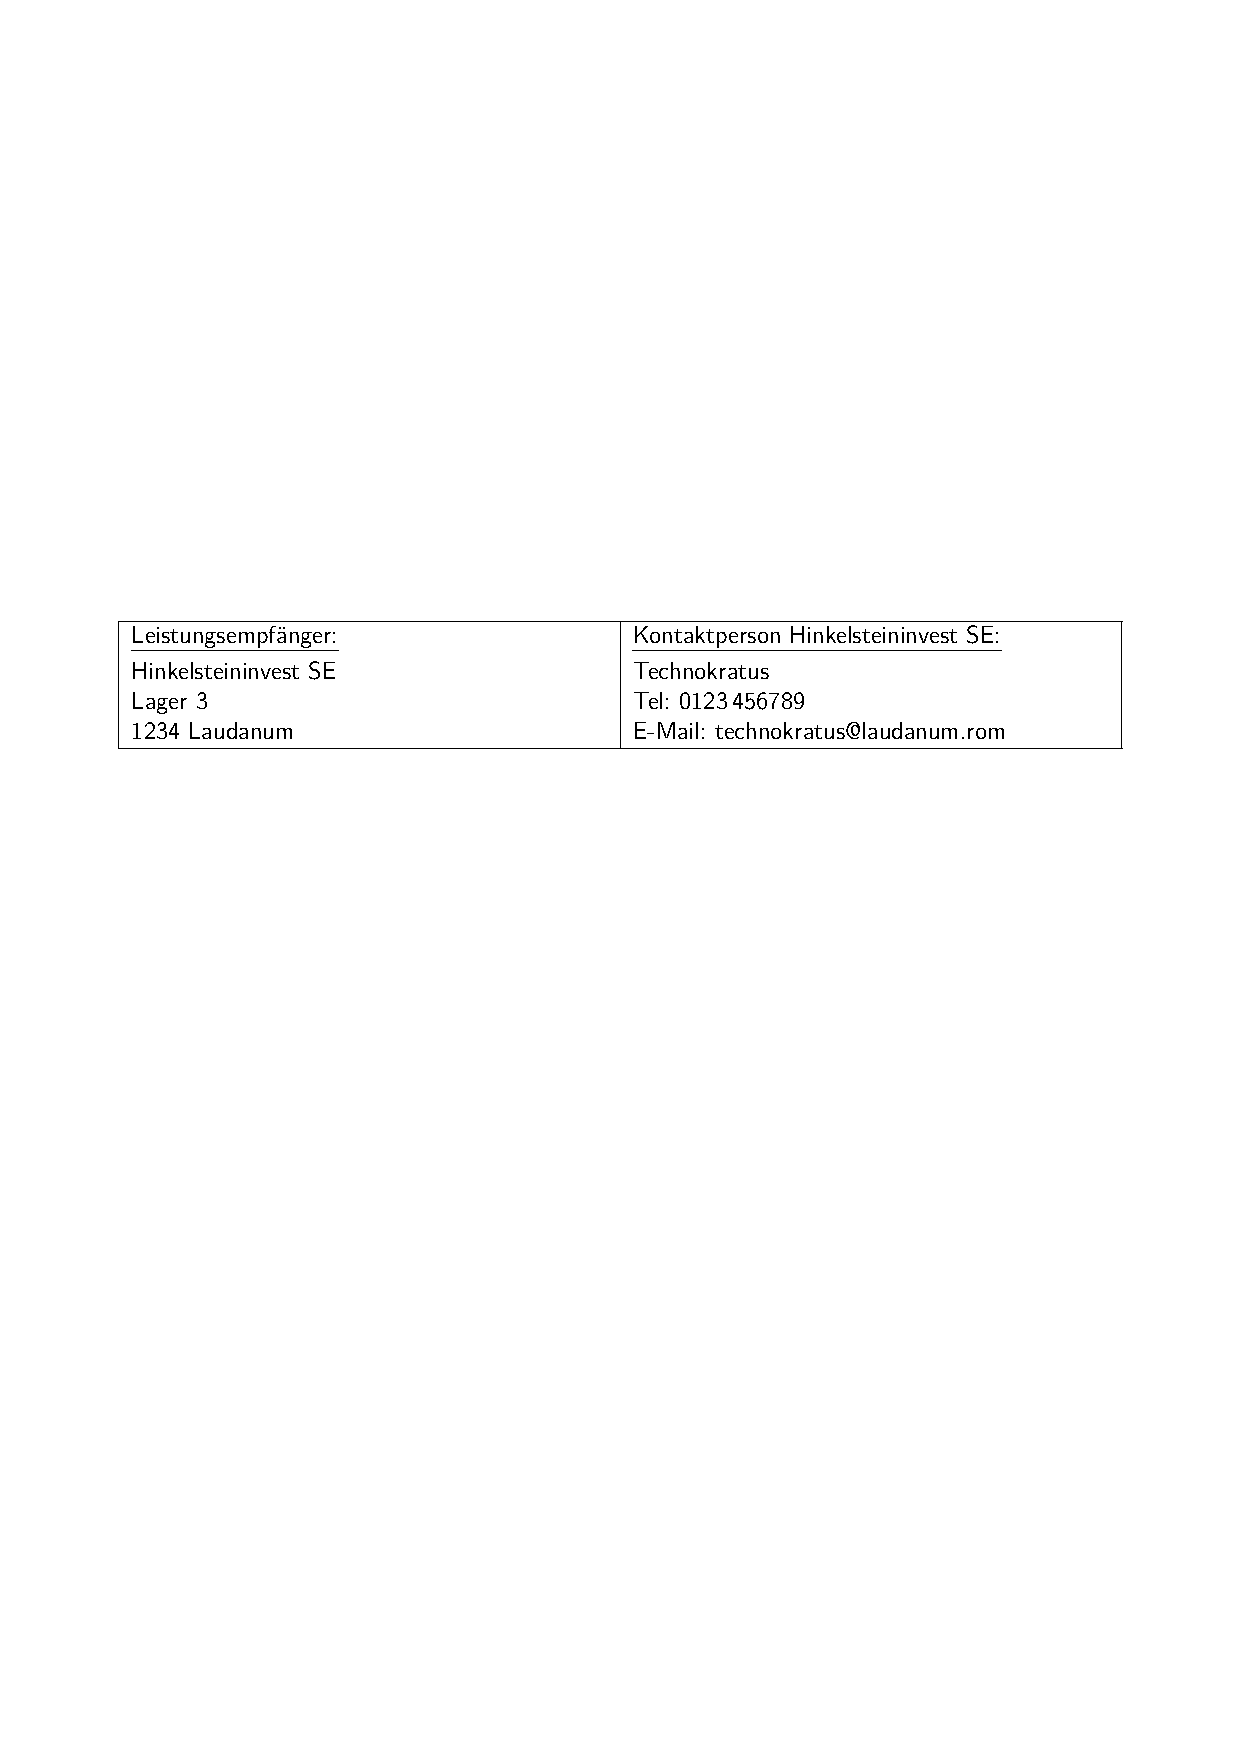
\includegraphics[height=2cm]{kundentabelle}

\vspace{-1em}

\caption{Tabelle mit Kundendaten -- gesteuert über \Cmd{kundentabelle}}
\label{kundentab}
\end{center}
\end{figure}

Schließlich kann noch mittels \Cmd{umsatzsteuer} die Höhe der Umsatzsteuer in Prozent angegeben werden. Der Wert wird später in der Berechnungen der Gesamtsumme benötigt.

\subsection{Firmendaten}

Es folgen nun die Angeben zur Firma, welche die Rechnung stellt. Es sind nicht alle Angaben zwingend notwendig. Ein Kommando darf jedoch in keinem Fall gelöscht werden. Sollen bestimmte Daten nicht auf der Rechnung erscheinen, kann beim entsprechenden Kommando die geschweifte Klammer leer bleiben.

\begin{verbatim}
% Firmendaten
\firmenname{Obelix GmbH \& Co. KG}
\firmenzusatz{}
\firmenanschrift{Am Steinbruch 1}
\firmenort{Kleines gallisches Dorf}
\firmenland{Aremorica}
\firmenwww{www.hinkelstein.ix}
\firmenemail{info@hinkelstein.ix}
\firmentel{1976\,/\,1978\,-\,0}
\firmenfax{1976\,/\,1978\,-\,23}
\firmenmobil{}
\firmeniban{IX11920518925000123}
\firmenbic{GENOIXH1AOI}
\firmenbank{Gallische Bank Lutetia}
\end{verbatim}

Die Kommandos sind selbsterklärend und werden an dieser Stelle nicht weiter erläutert. Ein Hinweis zu den Telefon- und Faxnummern: die Zeichenfolge \Cmd{,} fügt ein kurzes Leerzeichen ein.

\subsection{Kundendaten}

Entsprechend den Firmendaten oben folgen nun die Daten des Kunden. Auch diese Kommandos dürfen nur leer gelassen, nicht jedoch gelöscht werden.

\begin{verbatim}
% Kundendaten
\kundenname{Hinkelsteininvest SE}
\kundenzusatz{- Abteilung Ankauf -}
\kundenanschrift{Lager 3}
\kundenort{1234 Laudanum}
\kundenland{Aremorica}
\kundenkontakt{Technokratus}
\kundentel{0123\,456789}
\kundenemail{technokratus@laudanum.rom}
\end{verbatim}

Auch hier wird aufgrund der selbsterklärenden Kommandos nicht weiter auf diese eingegangen.

\subsection{Rechnungsdaten}

Als letztes werden nun im Dokumentkopf die Daten zur Rechnung angegeben. Diese erscheinen in einem Kasten rechts oben auf der Rechnung (Abbildung~\ref{rechtab}).

\begin{figure}[htbp]
\begin{center}
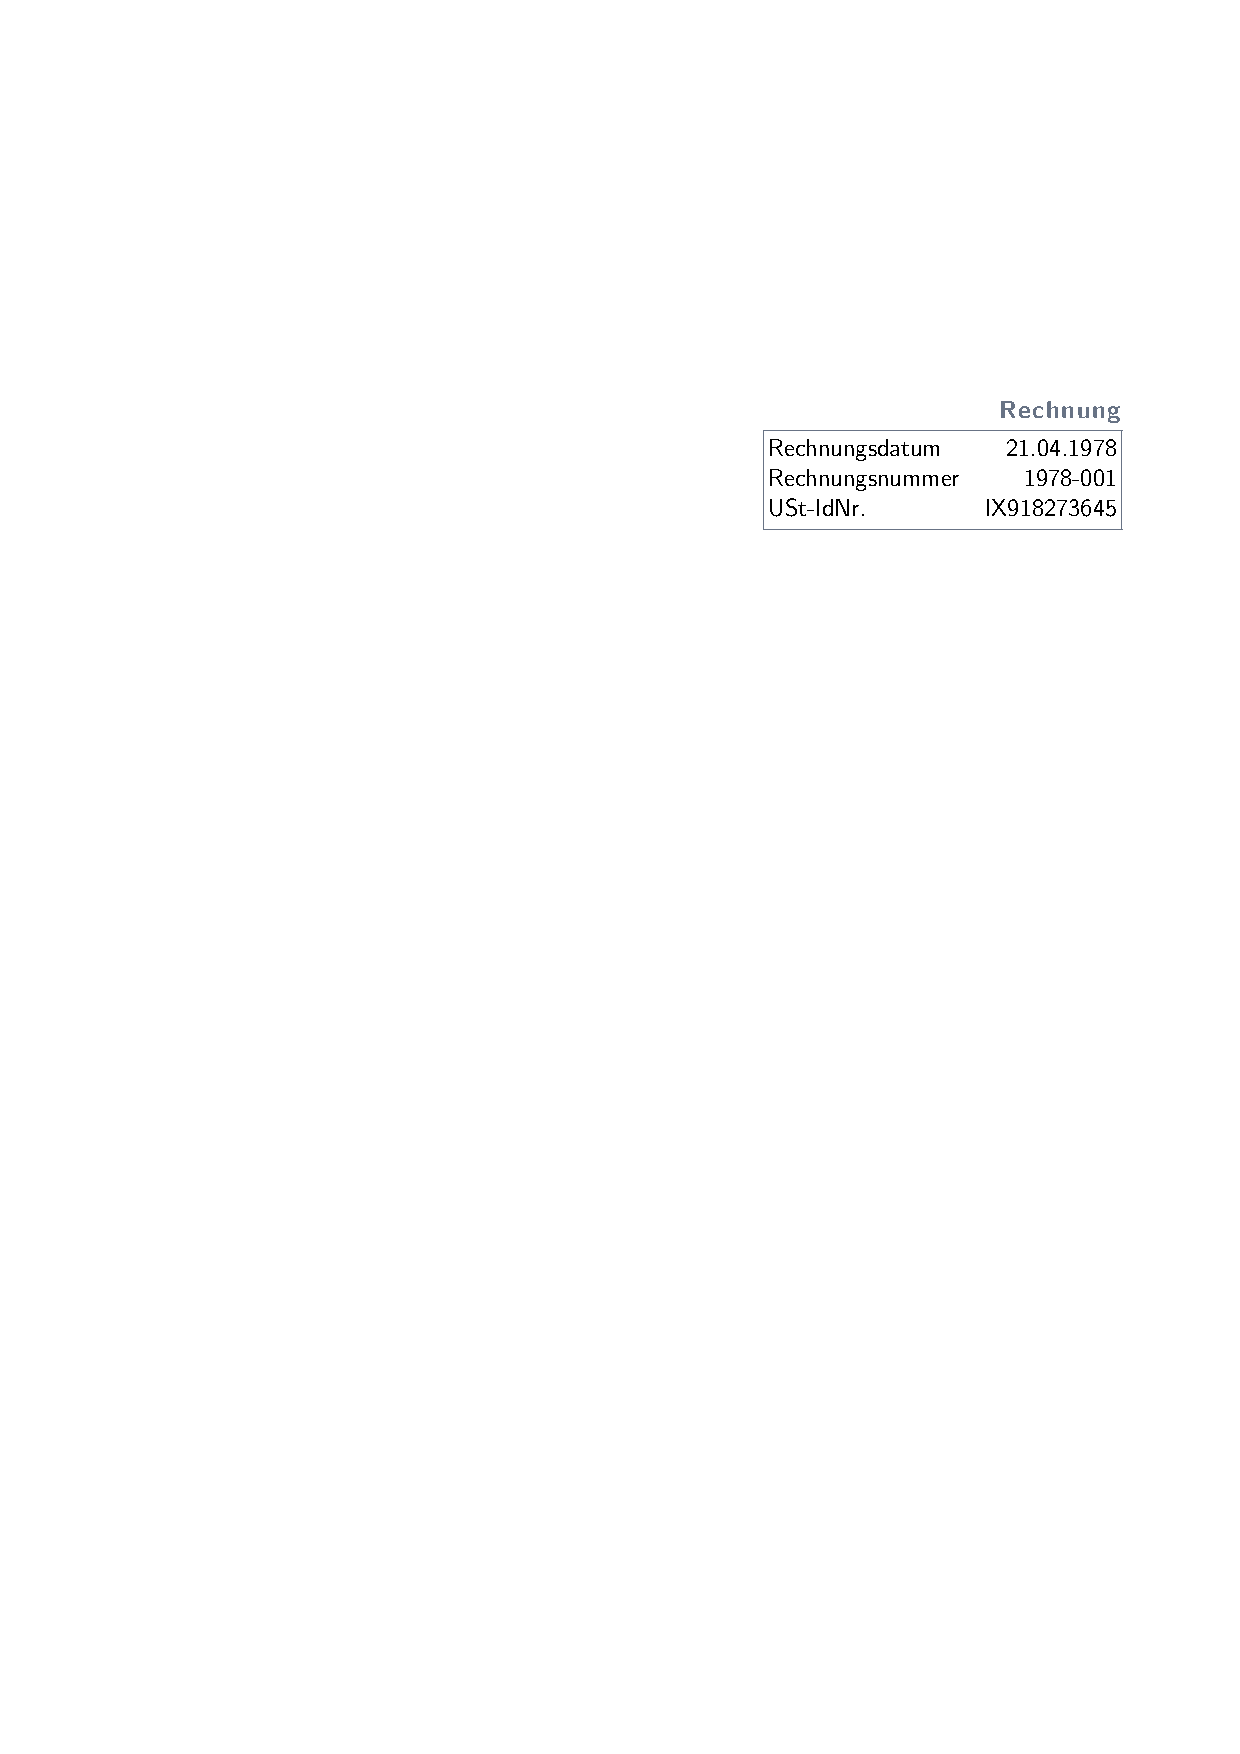
\includegraphics[height=2cm]{rechnungstabelle}

\vspace{-1em}

\caption{Box mit Rechnungsdaten}
\label{rechtab}
\end{center}
\end{figure}

\begin{verbatim}
% Rechnungsdaten
\rechnungsdatum{21.04.1978} % \heute = heutiges Datum
\rechnungsnummer{1978-001}
\ustnummer{IX918273645}
\end{verbatim}

Die Kommandos sind wieder selbsterklärend. Das Rechnungsdatum kann entweder statisch angegeben werden, z.\,B. als ,,21.04.1978``. Oder es wird das Kommando \Cmd{heute} genutzt um das aktuelle Datum einzufügen.

\section{Dokumentinhalt}

\subsection{Tabellen}

Der eigentliche Inhalt des Dokuments wird durch die beiden Kommandos \Cmd{begin\{document\}} und \Cmd{end\{document\}} eingeschlossen. Neben Text und sonstigen allgemeinen Inhalten können spezielle Kommandos genutzt werden, um standardisierte Rechnungstabellen einzufügen. Diese werden nachfolgend erläutert.

\begin{verbatim}
% Rechnungstext
\begin{document}
Sehr geehrte Damen und Herren,

ich erlaube mir entsprechend meiner erbrachten Leistung folgenden Betrag in Rechnung zu stellen:

\vspace{10mm}

\begin{tableistung}
\leistung{Planung Hinkelstein}{02.1978}{14}{20}
\leistung{Produktion Hinkelstein Prototyp\newline(Maßstab 1:10)}{02.1978}{6}{20}
\leistung{Serienproduktion\newline(Charge 1 -- 25 Stück)}{03.1978}{125}{20}
\end{tableistung}

\zwischensumme

\begin{tabreise}
\reise{Gallisches Dorf--Lutetia}{1}{450}{0.3}
\reise{Lutetia--Gallisches Dorf}{1}{450}{0.3}
\end{tabreise}

\begin{tabnacht}
\nacht{Mannekenpix}{24.01.--25.01.1978}{65}
\end{tabnacht}

\begin{tabsonstiges}
\sonstiges{Verladung}{100}
\sonstiges{Lieferung ab Werk}{250}
\end{tabsonstiges}

\gesamtbetrag{}

\end{document}
\end{verbatim}

\newpage

Es sind vier Tabellentypen vordefiniert (Tabelle~\ref{tabtab}). Diese sind als Umgebungen angelegt, d.\,h. der Inhalt wird jeweils von \Cmd{begin}- und \Cmd{end}- Kommandos eingeschlossen. Die einzelnen Tabellenzeilen werden wiederum durch ein weiteres Kommando eingefügt.
\begin{table}[htbp]
\caption{Tabellentypen}

\begin{center}
\begin{tabular}{llll}
\hline
Name&Typ&Zeilen-Kommando&Beispiel\\
\hline
tableistung&Leistungsabrechnung&\Cmd{leistung}&Abbildung~\ref{tab}a\\
tabreise&Reiseabrechnung&\Cmd{reise}&Abbildung~\ref{tab}b\\
tabnacht&Übernachtungsabrechnung&\Cmd{nacht}&Abbildung~\ref{tab}c\\
tabsonstiges&Abrechnung Sonstiges&\Cmd{sonstiges}&Abbildung~\ref{tab}d\\
\hline
\end{tabular}
\end{center}
\label{tabtab}
\end{table}%

\begin{figure}[htbp]
\begin{center}
\fbox{
\begin{tabularx}{15.5cm}{cm{15cm}}
a)&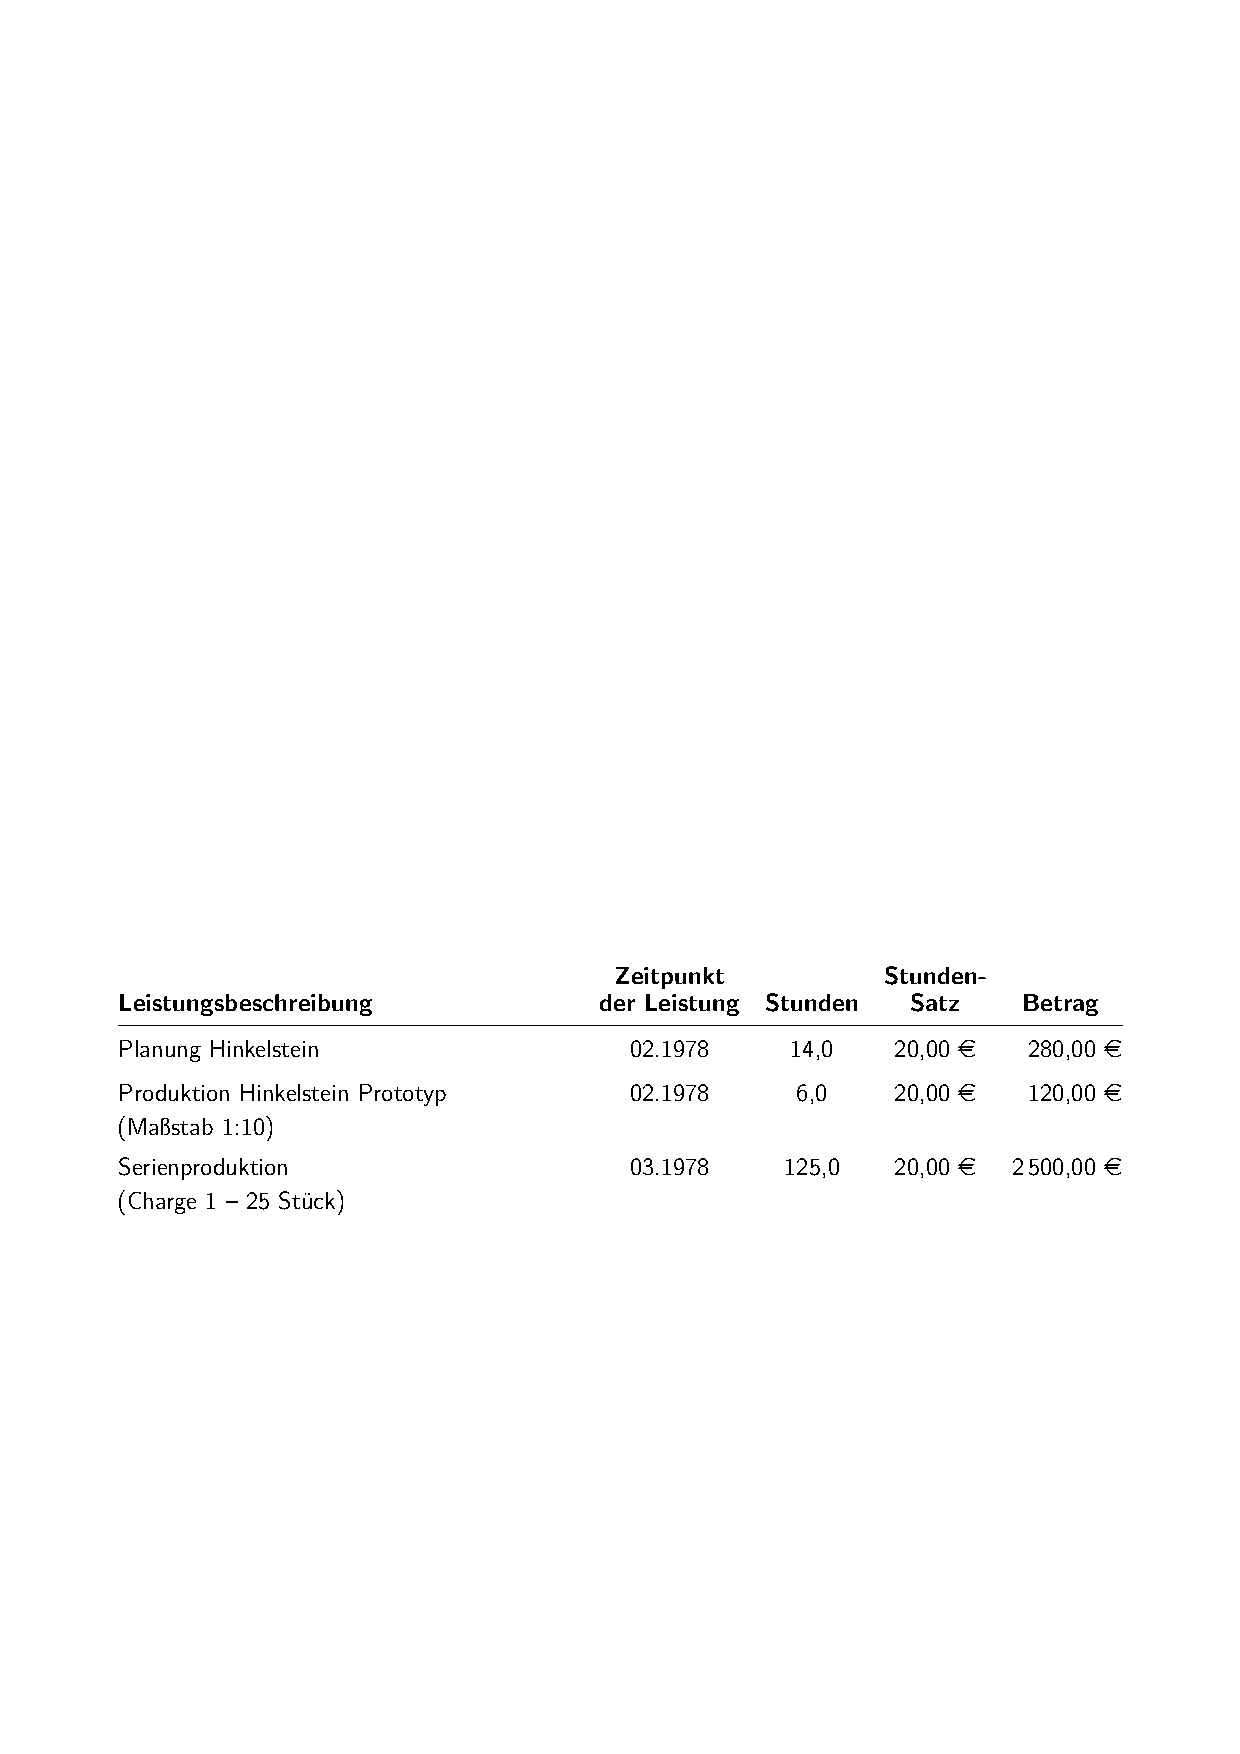
\includegraphics[width=14.2cm]{leisttab}\\[1.2em]
b)&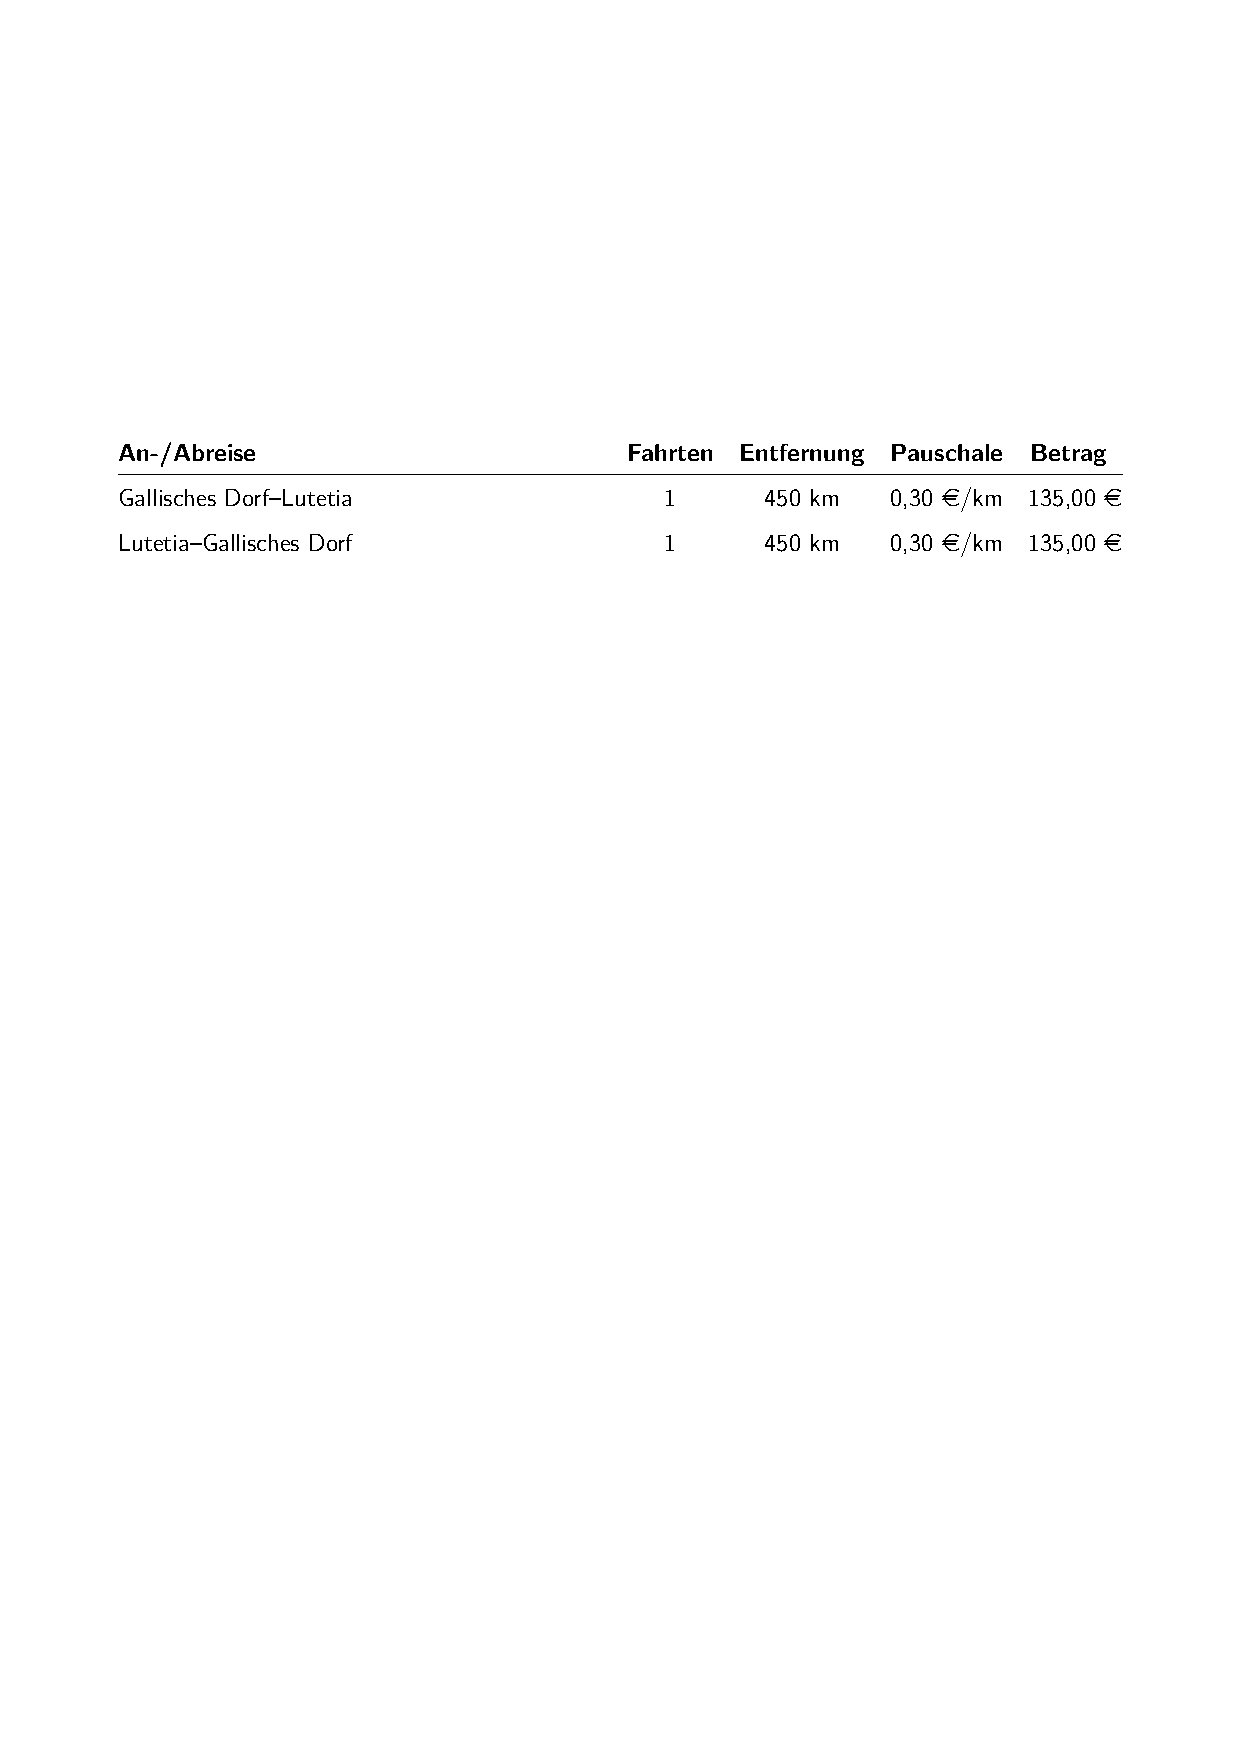
\includegraphics[width=14.2cm]{reisetab}\\[1.2em]
c)&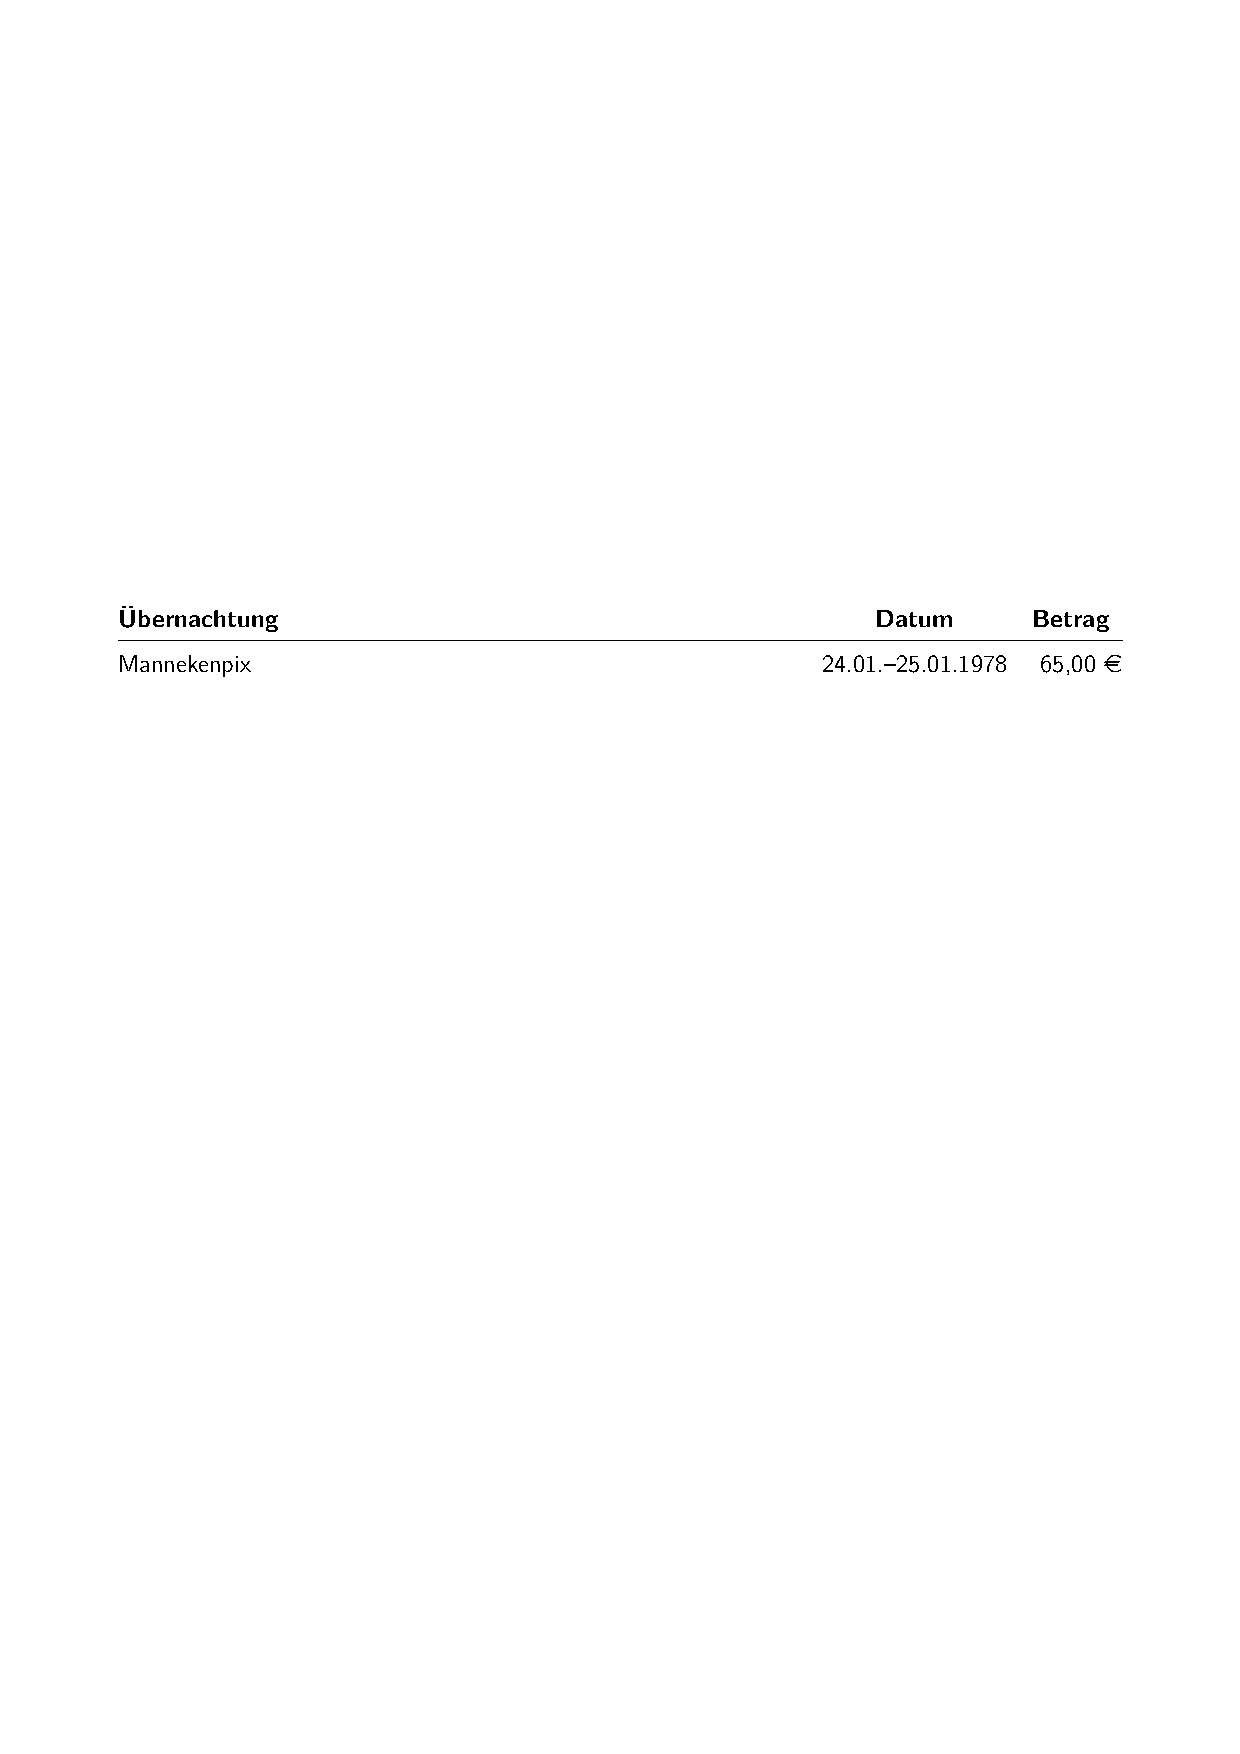
\includegraphics[width=14.2cm]{nachttab}\\[1.2em]
d)&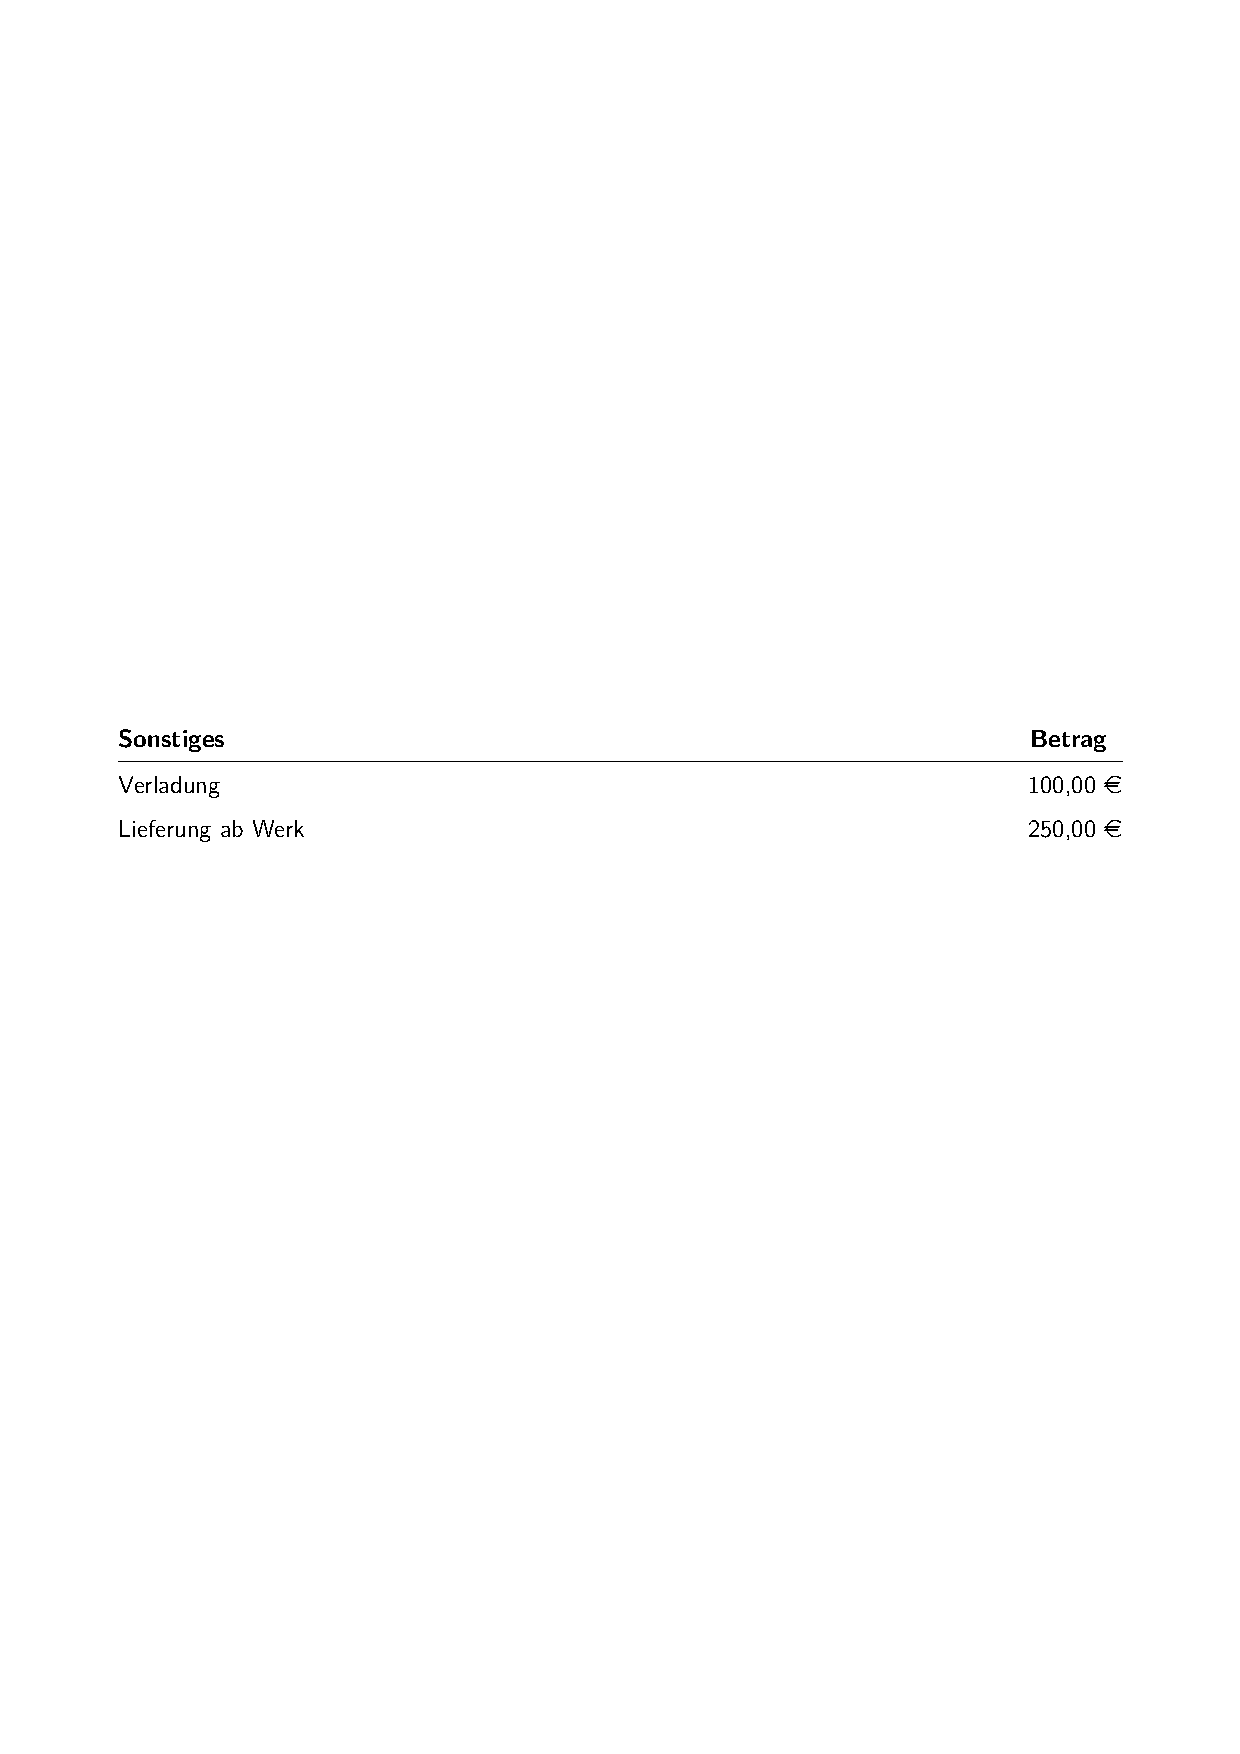
\includegraphics[width=14.2cm]{sonsttab}
\end{tabularx}
}

\vspace{-.5em}

\caption{Tabellenbeispiele: a) tableistung, b) tabreise, c) tabnacht und d) tabsonstiges}
\label{tab}
\end{center}
\end{figure}

Tabelle~\ref{zeiletab} zeigt eine Übersicht über die Argumente der Zeilen-Kommandos. Diese können innerhalb der jeweiligen Tabellenumgebung unbegrenzt oft eingesetzt werden. Auch die Tabellen\-umgebungen selbst können mehr als einmal eingefügt werden, um beispielsweise verschiedene detaillierte Leistungspakete in mehrere Tabellen aufzuteilen.
\begin{table}[htb]
\caption{Argumente der Zeilen-Kommandos}

\begin{center}
\begin{tabular}{lllll}
\hline
Kommando&Argument 1&Argument 2&Argument 3&Argument 4\\
\hline
\Cmd{leistung}&Leistungsbeschreibung&Zeitpunkt&Stundenanzahl&Stundensatz\\
\Cmd{reise}&Reisebeschreibung&Fahrtanzahl&Entfernung&Pauschale\\
\Cmd{nacht}&Unterkunft&Datum&Betrag&--\\
\Cmd{sonstiges}&Beschreibung&Betrag&--&--\\
\hline
\end{tabular}
\end{center}
\label{zeiletab}
\end{table}% 

\vspace{1em}

Drei Hinweise zu hilfreichen \LaTeX-Kommandos: Mittels \Cmd{vspace\{\}} kann ein vertikaler Zwischenraum (angegeben z.\,B. in mm oder cm) eingefügt werden. Mit dem Kommando \Cmd{newline} wird ein Zeilen\-umbruch innerhalb einer Tabellenzelle eingefügt (siehe tableistung im Beispiel). Ein Bis-Strich, wie in 24.02.--25.02.2014, wird durch zwei aufeinanderfolgende, einfache Bindestriche (\verb|--|) erzeugt. 

\subsection{Zwischensummen und Gesamtbeträge}

Die Vorlage bietet die Möglichkeit neben dem Gesamtrechnungsbetrag auch Zwischensummen in die Rechnung einzufügen. Zwischensummen erzeugen immer einen Seitenumbruch und einen anschließenden Übertrag. Sie werden durch das Kommando \Cmd{zwischensumme} zwischen zwei Tabellenumgebungen eingefügt. Abbildung~\ref{zwischtab}.

\begin{figure}[htbp]
\begin{center}
\fbox{
\begin{tabularx}{15.5cm}{cm{15cm}}
a)&
\includegraphics[width=14.2cm]{zwischtab}\\[1.2em]
b)&
\includegraphics[width=14.2cm]{uebertab}
\end{tabularx}
}

\vspace{-.5em}

\caption{Beispiel für a) Zwischensumme und b) Übertrag, erzeugt mit \Cmd{zwischensumme}}
\label{zwischtab}
\end{center}
\end{figure}

Der Gesamtbetrag der Rechnung wird mit dem Kommando \Cmd{gesamtbetrag\{\}} eingefügt. Wurde bereits eine Anzahlung geleistet, die vom Bruttobetrag abgezogen werden soll, kann dieser Teilbetrag als Argument in den geschweiften Klammern angegeben werden (Abbildung~\ref{gesamttab}b). Um einen normalen Rechnungsgesamtbetrag zu erzeugen bleiben die geschweiften Klammern leer (Abbildung~\ref{gesamttab}a).

\begin{figure}[htbp]
\begin{center}
\fbox{
\begin{tabularx}{15.5cm}{cm{15cm}}
a)&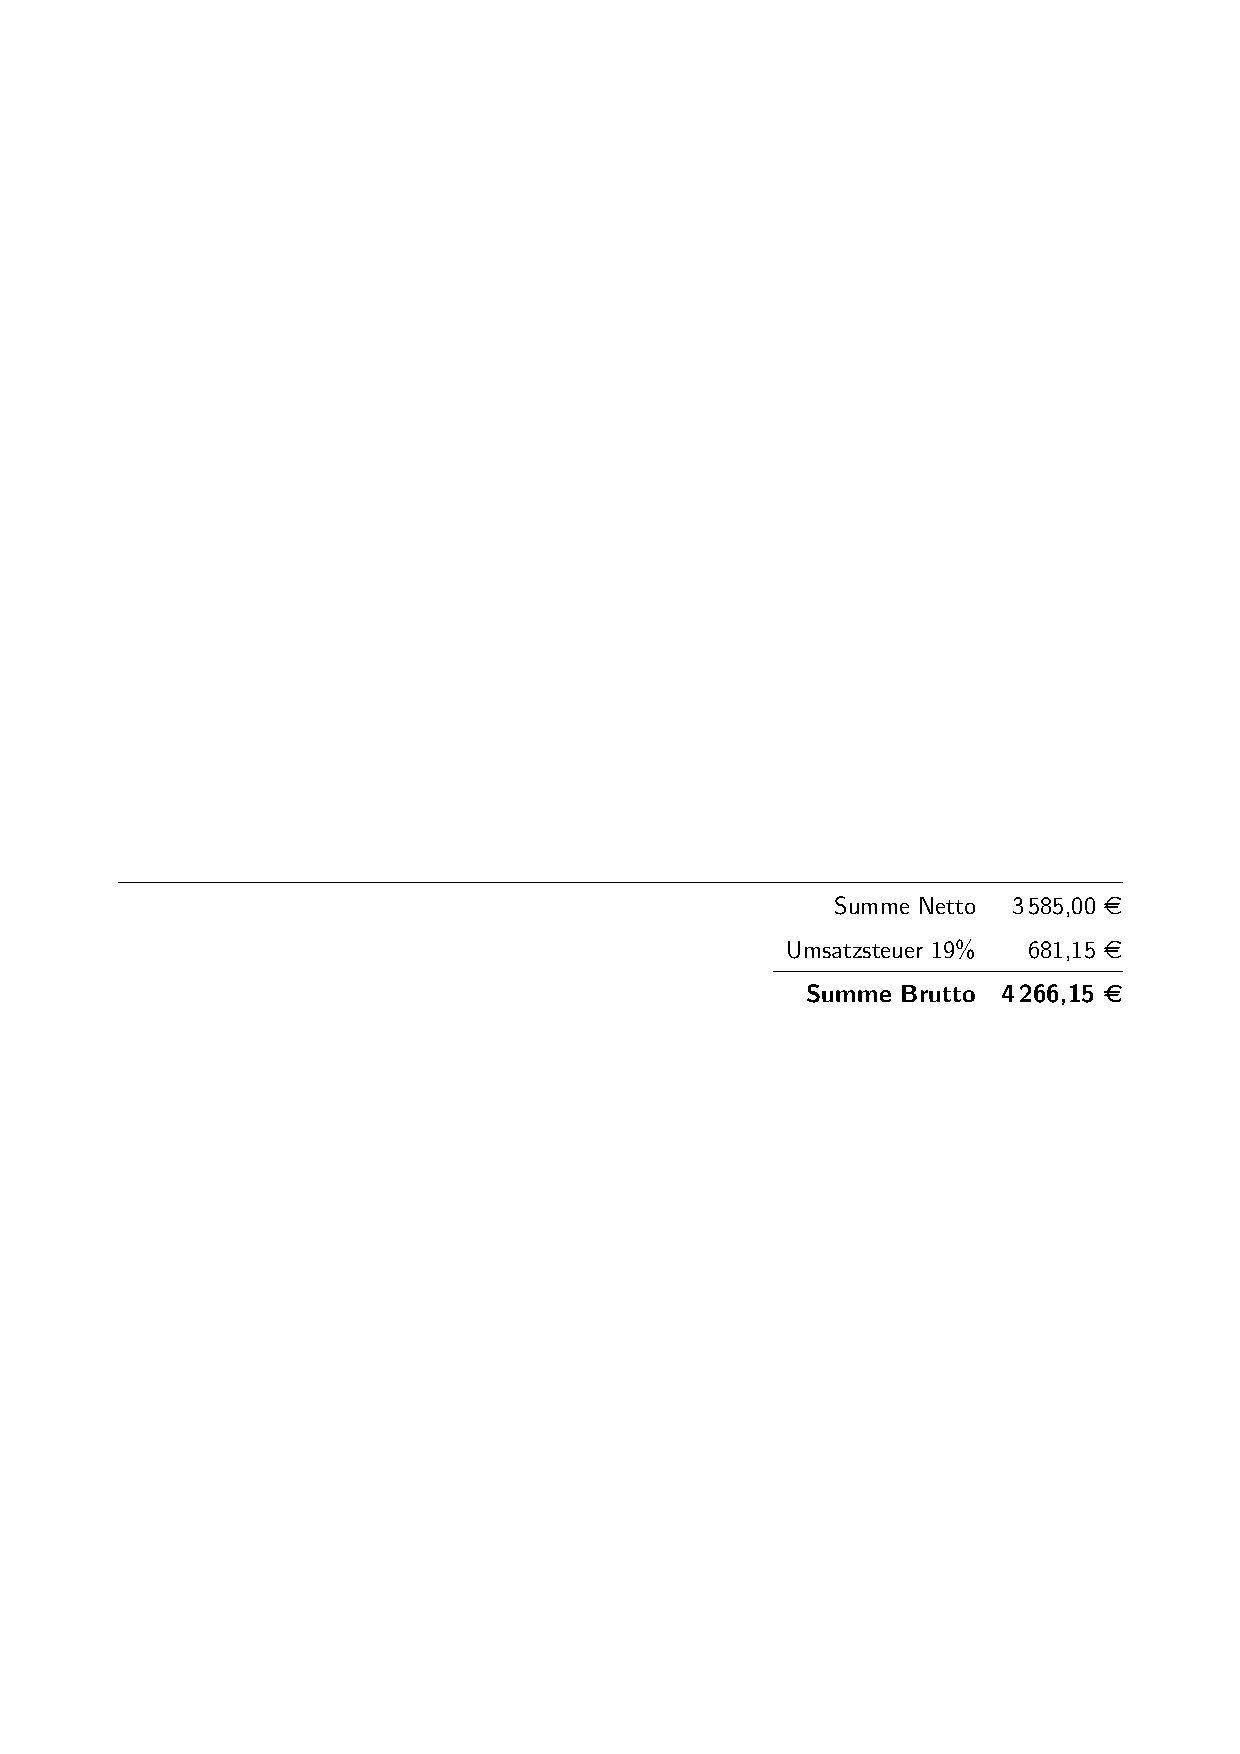
\includegraphics[width=14.2cm]{gesamttab}\\[1.2em]
b)&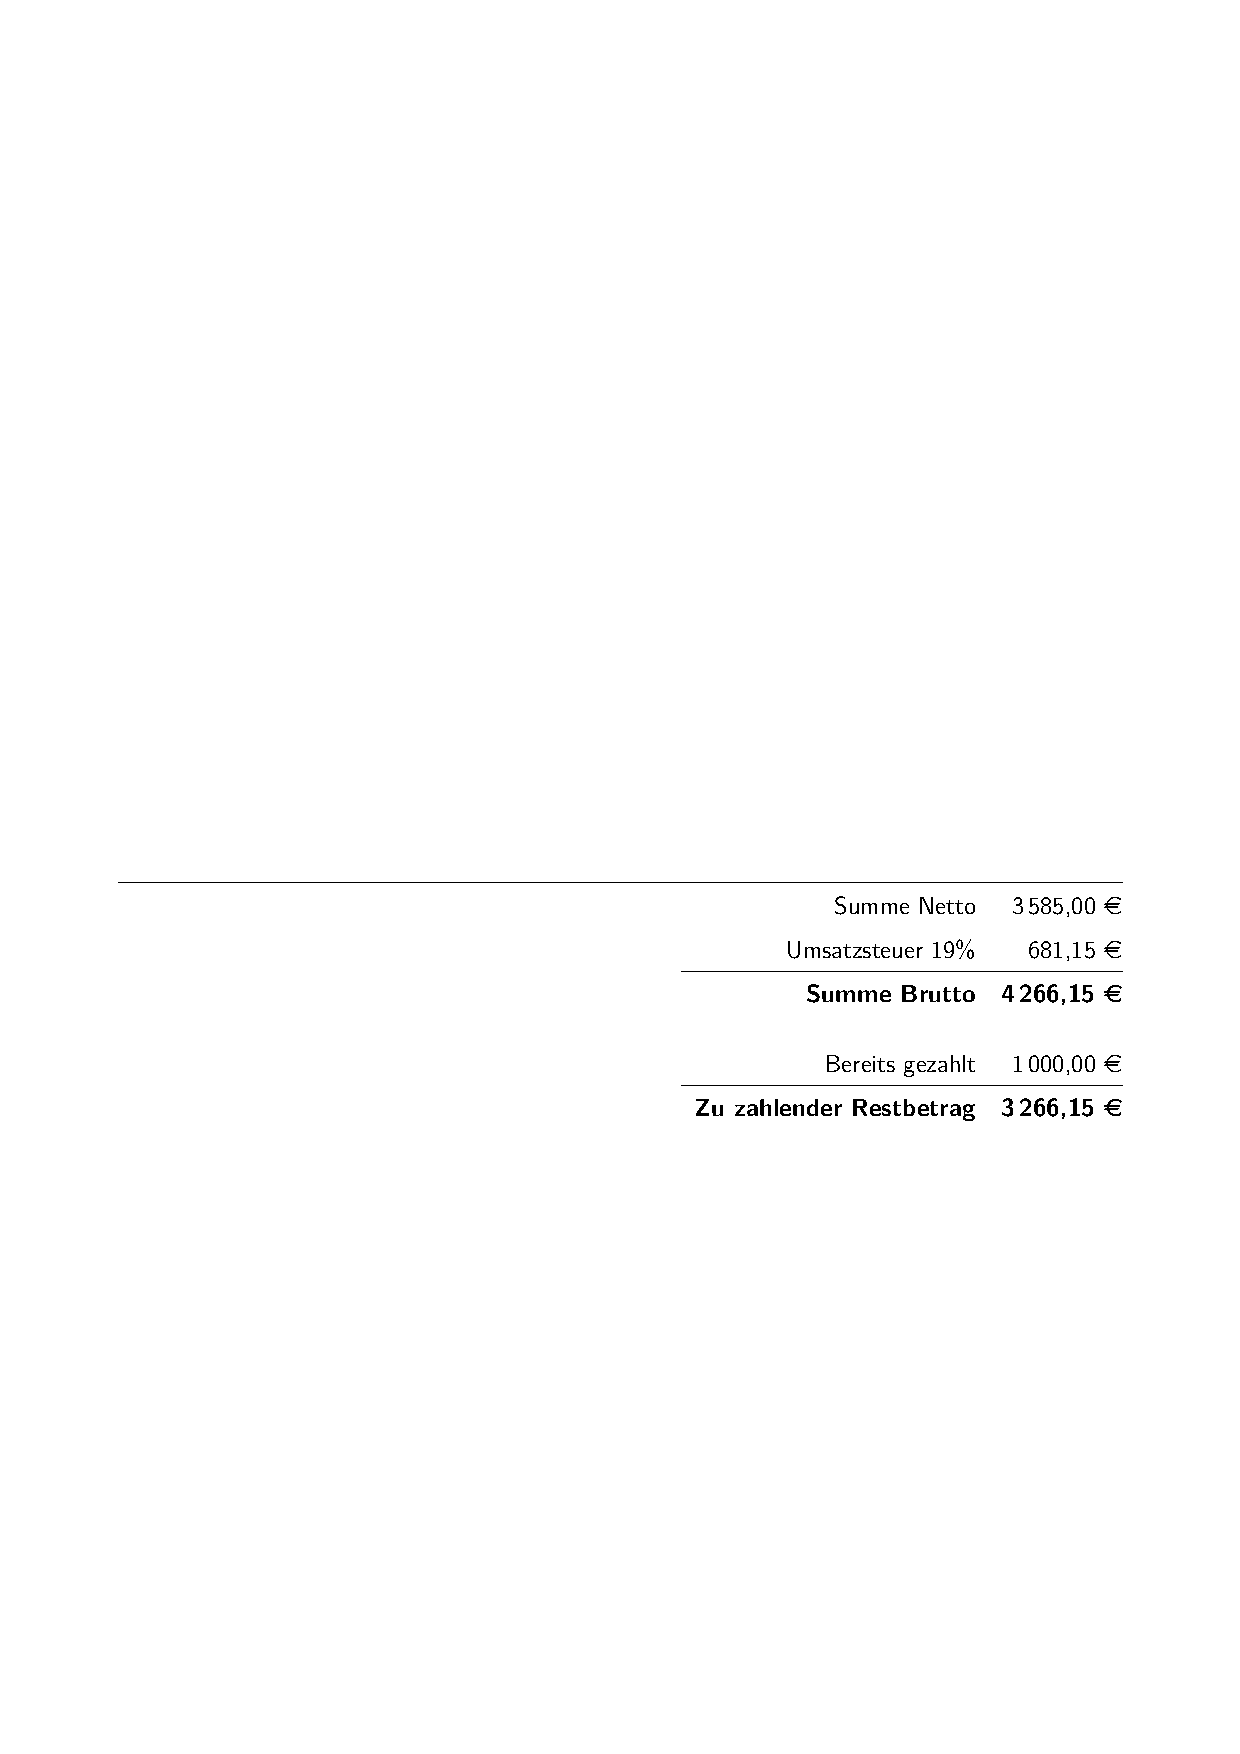
\includegraphics[width=14.2cm]{teiltab}
\end{tabularx}
}

\vspace{-.5em}

\caption{Beispiel für den Gesamtbetrag, erzeugt mittels a) \Cmd{gesamtbetrag\{\}}} und b) mit bereits angezahltem Teilbetrag durch \Cmd{gesamtbetrag\{1000\}}
\label{gesamttab}
\end{center}
\end{figure}

\end{document}
